\section[Abordagem de Orienta��o]{Abordagem de Orienta��o}

\begin{frame}
    \frametitle{Intelig�ncia de enxames}

    \begin{itemize}
        \item <1-> Estudos sobre col�nias de insetos (formigas, cupins, abelhas,
        etc);
        \item <2-> Agentes simples interagindo entre si;
        \item <3-> Insetos isoladamente n�o t�m um comportamento
        relevante;
        \item <4-> Em grupo revelam-se uma organiza��o bastante complexa.
    \end{itemize}
\end{frame}

\begin{frame}
    \frametitle{Abordagem de Orienta��o}
    \begin{itemize}

        %\item <1-> capacidade de auto-organiza��o: estigmergia;

        \item <1-> Paradigma de heur�sticas construtivas: \emph{Ant Colony Optimization}
        (ACO) \cite{dorigo:96};

        \item <2-> Formigas reais comunicam-se indiretamente:
        \emph{ferom�nio};

        \item <3-> Fun��o do indiv�duo: procura e o transporte do alimento da fonte at� o
        formigueiro;
        \item <4-> Escolha do caminho: maior quantidade de ferom�nio;
        \item <5-> Em pouco tempo o menor caminho entre origem e
        destino � estabelecido.

    \end{itemize}
\end{frame}

\begin{frame}
    \frametitle{Formigas Reais em Busca de Alimento}

    \begin{figure}[htb]
        \begin{center}
            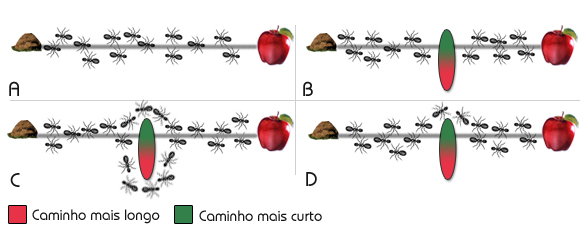
\includegraphics[width=\textwidth]{images/aco/formigas.jpg}
            \caption{Formigas em busca de alimento encontram o menor caminho entre alimento e ninho}
        \end{center}
        \label{fig:formigas}
    \end{figure}

\end{frame}
